\documentclass{article}

%----------------------------------------------------------------------------------------
%	PACKAGES AND OTHER DOCUMENT CONFIGURATIONS
%----------------------------------------------------------------------------------------

\usepackage{amsmath,amsfonts,stmaryrd,amssymb} % Math packages
\usepackage{enumerate} % Custom item numbers for enumerations
\usepackage[ruled]{algorithm2e} % Algorithms
\usepackage[framemethod=tikz]{mdframed} % Allows defining custom boxed/framed environments
\usepackage{textcomp}
\usepackage{float}
\usepackage{biblatex}
\usepackage{listings} % File listings, with syntax highlighting
\usepackage{graphicx}
\usepackage{hyperref}

\makeatletter
\newcommand{\addloflink}[1]{% \addloflink{<URL>}
  \addtocontents{lof}{\begingroup\def\protect\@dotsep{10000}% Remove dots in LoF for this entry
    \protect\contentsline{figlink}{\protect\numberline{}\url{#1}}{}{}%
    \endgroup}% Restore dots in LoF for future entries
}


%----------------------------------------------------------------------------------------
%	DOCUMENT MARGINS
%----------------------------------------------------------------------------------------

\usepackage{geometry} % Required for adjusting page dimensions and margins

\geometry{
	paper=a4paper, % Paper size, change to letterpaper for US letter size
	top=2.5cm, % Top margin
	bottom=3cm, % Bottom margin
	left=2.5cm, % Left margin
	right=2.5cm, % Right margin
	headheight=14pt, % Header height
	footskip=1.5cm, % Space from the bottom margin to the baseline of the footer
	headsep=1.2cm, % Space from the top margin to the baseline of the header
	%showframe, % Uncomment to show how the type block is set on the page
}

%----------------------------------------------------------------------------------------
%	FONTS
%----------------------------------------------------------------------------------------

\usepackage[utf8]{inputenc} % Required for inputting international characters
\usepackage[T1]{fontenc} % Output font encoding for international characters

\usepackage{XCharter} % Use the XCharter fonts

%----------------------------------------------------------------------------------------
%	COMMAND LINE ENVIRONMENT
%----------------------------------------------------------------------------------------

% Usage:
% \begin{commandline}
%	\begin{verbatim}
%		$ ls
%		
%		Applications	Desktop	...
%	\end{verbatim}
% \end{commandline}

\mdfdefinestyle{commandline}{
	leftmargin=10pt,
	rightmargin=10pt,
	innerleftmargin=15pt,
	middlelinecolor=black!50!white,
	middlelinewidth=2pt,
	frametitlerule=false,
	backgroundcolor=black!5!white,
	frametitle={Command Line},
	frametitlefont={\normalfont\sffamily\color{white}\hspace{-1em}},
	frametitlebackgroundcolor=black!50!white,
	nobreak,
}

% Define a custom environment for command-line snapshots
\newenvironment{commandline}{
	\medskip
	\begin{mdframed}[style=commandline]
}{
	\end{mdframed}
	\medskip
}

%----------------------------------------------------------------------------------------
%	FILE CONTENTS ENVIRONMENT
%----------------------------------------------------------------------------------------

% Usage:
% \begin{file}[optional filename, defaults to "File"]
%	File contents, for example, with a listings environment
% \end{file}

\mdfdefinestyle{file}{
	innertopmargin=1.6\baselineskip,
	innerbottommargin=0.8\baselineskip,
	topline=false, bottomline=false,
	leftline=false, rightline=false,
	leftmargin=2cm,
	rightmargin=2cm,
	singleextra={%
		\draw[fill=black!10!white](P)++(0,-1.2em)rectangle(P-|O);
		\node[anchor=north west]
		at(P-|O){\ttfamily\mdfilename};
		%
		\def\l{3em}
		\draw(O-|P)++(-\l,0)--++(\l,\l)--(P)--(P-|O)--(O)--cycle;
		\draw(O-|P)++(-\l,0)--++(0,\l)--++(\l,0);
	},
	nobreak,
}

% Define a custom environment for file contents
\newenvironment{file}[1][File]{ % Set the default filename to "File"
	\medskip
	\newcommand{\mdfilename}{#1}
	\begin{mdframed}[style=file]
}{
	\end{mdframed}
	\medskip
}

%----------------------------------------------------------------------------------------
%	NUMBERED QUESTIONS ENVIRONMENT
%----------------------------------------------------------------------------------------

% Usage:
% \begin{question}[optional title]
%	Question contents
% \end{question}

\mdfdefinestyle{question}{
	innertopmargin=1.2\baselineskip,
	innerbottommargin=0.8\baselineskip,
	roundcorner=5pt,
	nobreak,
	singleextra={%
		\draw(P-|O)node[xshift=1em,anchor=west,fill=white,draw,rounded corners=5pt]{%
		Question \theQuestion\questionTitle};
	},
}

\newcounter{Question} % Stores the current question number that gets iterated with each new question

% Define a custom environment for numbered questions
\newenvironment{question}[1][\unskip]{
	\bigskip
	\stepcounter{Question}
	\newcommand{\questionTitle}{~#1}
	\begin{mdframed}[style=question]
}{
	\end{mdframed}
	\medskip
}

%----------------------------------------------------------------------------------------
%	WARNING TEXT ENVIRONMENT
%----------------------------------------------------------------------------------------

% Usage:
% \begin{warn}[optional title, defaults to "Warning:"]
%	Contents
% \end{warn}

\mdfdefinestyle{warning}{
	topline=false, bottomline=false,
	leftline=false, rightline=false,
	nobreak,
	singleextra={%
		\draw(P-|O)++(-0.5em,0)node(tmp1){};
		\draw(P-|O)++(0.5em,0)node(tmp2){};
		\fill[black,rotate around={45:(P-|O)}](tmp1)rectangle(tmp2);
		\node at(P-|O){\color{white}\scriptsize\bf !};
		\draw[very thick](P-|O)++(0,-1em)--(O);%--(O-|P);
	}
}

% Define a custom environment for warning text
\newenvironment{warn}[1][Warning:]{ % Set the default warning to "Warning:"
	\medskip
	\begin{mdframed}[style=warning]
		\noindent{\textbf{#1}}
}{
	\end{mdframed}
}

%----------------------------------------------------------------------------------------
%	INFORMATION ENVIRONMENT
%----------------------------------------------------------------------------------------

% Usage:
% \begin{info}[optional title, defaults to "Info:"]
% 	contents
% 	\end{info}

\mdfdefinestyle{info}{%
	topline=false, bottomline=false,
	leftline=false, rightline=false,
	nobreak,
	singleextra={%
		\fill[black](P-|O)circle[radius=0.4em];
		\node at(P-|O){\color{white}\scriptsize\bf i};
		\draw[very thick](P-|O)++(0,-0.8em)--(O);%--(O-|P);
	}
}

% Define a custom environment for information
\newenvironment{info}[1][Info:]{ % Set the default title to "Info:"
	\medskip
	\begin{mdframed}[style=info]
		\noindent{\textbf{#1}}
}{
	\end{mdframed}
}


\usepackage{biblatex}
\usepackage{graphicx}

\bibliography{references}

\title{IHDCB339: Reading Notes}

\author{Kenny Warszawski\\ \texttt{kenny.warszawski@student.unamur.be}}

\date{University of Namur --- \today}

\begin{document}

\maketitle 

\section{Article Reference}

\textbf{Lam, An and Haugen, Øystein} "Complex Event Processing in ThingML", pp. 20-35, 2016.

\section{Overview}

The article is a presentation of a cross platform modelling language called \textit{ThingML} which is dedicated to Internet of Things. More precisely, the article focus on an extension of this language for Complex Event Processing (CEP). 

%----------------------------------------------------------------------------------------
%	General Problem
%----------------------------------------------------------------------------------------

\subsection{General problem}

Nowadays, Cyber Physical Systems (CPS) are increasingly present and need to have extremely fast responses. CEP is an answer to this constraint. Indeed, it allows the analysis and extraction of informations from an event sent from a transmitter and combine it with others in order to obtain more complex information on a system. ThingML helps the implementation of such complex system by adding an abstraction on the programming language used for deployment. That way, a model described in ThingML has the same behaviour even if it is deployed in Java or C/C++. This article treats the capabilities of ThingML with CEP extension to integrate a CEP system and deal with CPS constraints.

%----------------------------------------------------------------------------------------
%	CONCEPTS
%----------------------------------------------------------------------------------------

\section{Concepts used in the article}

\begin{itemize}
    \item \textbf{Complex Event Processing (CEP):} Complex Event Processing (CEP) is a set of methods and techniques for tracking
and analyzing real-time streams of information and detecting patterns or correlations
of unrelated data (complex events) that are of interest to a particular
business \cite{1}
	\item \textbf{Internet of Things (IoT):} The Internet of Things(IoT) is a novel paradigm that is rapidly gaining ground in the scenario of modern wireless telecommunications. The basic idea of this concept is the pervasive presence around us of a variety of things or objects – such as Radio-Frequency IDentification (RFID) tags, sensors, actuators, mobile phones, etc. – which,through unique addressing schemes, are able to interact with each other and cooperate with their neighbors to reach common goals \cite{2}
	\item \textbf{Event Pattern Language (EPL):} Event Pattern Language (EPL) is the language
to define atomic or complex event and specify the process of filtering (determine event of interest) and extracting events properties for constructing high-level events \cite{4}
	\item \textbf{Cyber Physical Systems (CPS):} Cyber-Physical Systems (CPS) are integrations of computation and physical processes. Embedded computers and networks monitor and control the physical processes, usually with feedback loops where physical processes affect computations and vice versa \cite{5}
	\item \textbf{RFID:} Radio Frequency Identification (RFID) is a wireless technology capable of automatic and unambiguous identification without line of sight by extracting a unique identifier from microelectronic tags attached to objects. \cite{3}
\end{itemize}

%----------------------------------------------------------------------------------------

\section{Article Summary}

\subsection{Thematic}

ThingML is a domain specific language and compiler for the internet of things. This DSL is used to describe software components and communication protocols without being coupled to a specific programming language. To this end, this technology provides the possibility for developers to deploy the same implementation onto different platforms like Java, Javascript, C/C++ and Arduino by a code generation.

\begin{figure}[h!]
	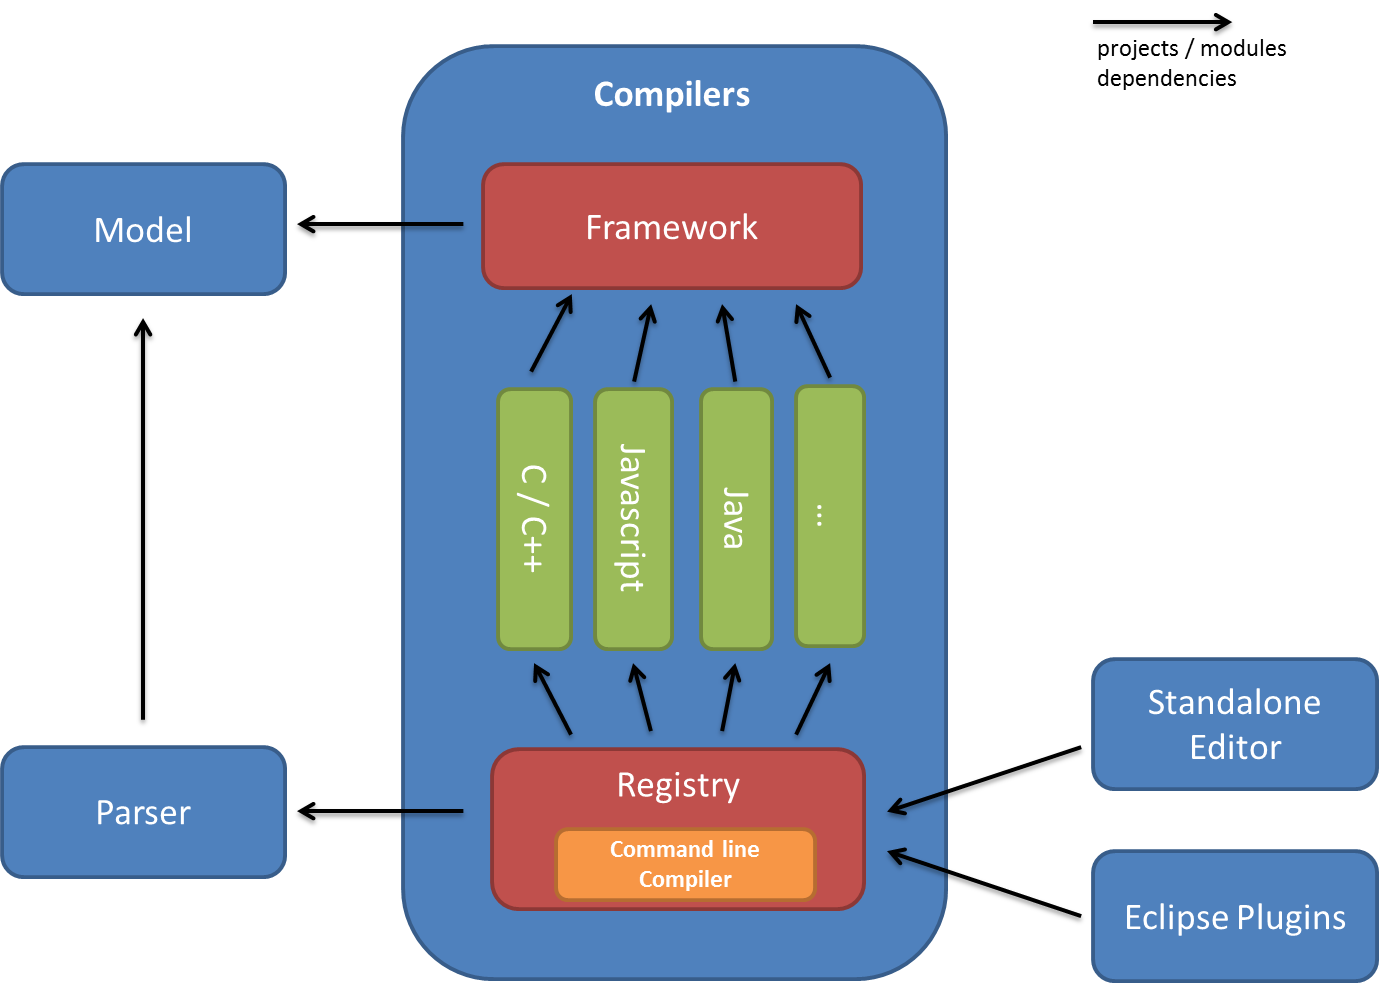
\includegraphics[width=\linewidth]{dsl.png}
	\caption{ThingML overview}
  	\label{fig:thingml} 
\end{figure}



%----------------------------------------------------------------------------------------

\section{Conclusions}


In malesuada ullamcorper urna, sed dapibus diam sollicitudin non. Donec elit odio, accumsan ac nisl a, tempor imperdiet eros. Donec porta tortor eu risus consequat, a pharetra tortor tristique. Morbi sit amet laoreet erat. Morbi et luctus diam, quis porta ipsum. Quisque libero dolor, suscipit id facilisis eget, sodales volutpat dolor. Nullam vulputate interdum aliquam. Mauris id convallis erat, ut vehicula neque. Sed auctor nibh et elit fringilla, nec ultricies dui sollicitudin. Vestibulum vestibulum luctus metus venenatis facilisis. Suspendisse iaculis augue at vehicula ornare. Sed vel eros ut velit fermentum porttitor sed sed massa. Fusce venenatis, metus a rutrum sagittis, enim ex maximus velit, id semper nisi velit eu purus.

\printbibliography

\end{document}
